\documentclass[11pt, final]{article}
\usepackage{mathpartir}
\usepackage{stmaryrd}
\usepackage{mathtools}
\usepackage{array,booktabs,ragged2e}
\usepackage[english]{babel}
\usepackage[utf8]{inputenc}
\usepackage{xfrac}
\usepackage{graphicx}
\usepackage{fancyhdr}
\usepackage{microtype}
\usepackage{glossaries}
% TODO: Setup symbol list
\usepackage[draft=false,cache]{minted}
\setlength{\marginparwidth}{3cm}
\usepackage{libertine}
\usepackage{dsfont}
% \usepackage{libertinust1math}
\usepackage{amssymb, amsthm, amsmath}
\usepackage{thmtools}
\usepackage[justification=centering]{caption}
\usepackage{csquotes}
\usepackage{etoolbox}
\usepackage{showkeys}
\usepackage[
  backend=biber,
  bibstyle=ieee,
  citestyle=ieee,
  sorting=ynt,
  hyperref=true,
  backref=true
]{biblatex}
% \usepackage[hidelinks]{hyperref}
\usepackage[hidelinks]{hyperref}
\usepackage{fontspec}
\setmainfont{TeX Gyre Pagella}
\setsansfont{TeX Gyre Heros}[Scale=MatchLowercase]
\setmonofont{Inconsolata}[Scale=MatchLowercase]
\RecustomVerbatimEnvironment{Verbatim}{BVerbatim}{}
\renewcommand{\figurename}{Listing}
\setminted[coq]{escapeinside=~~,mathescape}
\newcommand{\br}[1]{\langle #1 \rangle}
\def\Yields{\Downarrow}
\newcommand{\makefootnotelist}[1]{%
    \parbox{0.8\textwidth} {%
        \footnotesize{%
            \renewcommand*{\do}[1]{##1\\}%
            \dolistcsloop{#1}}}}%
\newcommand{\fancyfootnote}[1]{%
    \footnotemark{}%
    \def\listname{footlist\thepage}%
    \def\n{$^{\the\numexpr\value{footnote}}$}
    \ifcsdef{\listname}%
        {\listcseadd{\listname}{\n\ #1}}%
        {\csedef{\listname}{}%
        \listcseadd{\listname}{\n\ #1}}%
    \fancypagestyle{fancyfootnote}{%
        \fancyfoot[L]{\makefootnotelist{\listname}}%
        \fancyfoot[C]{}%
        \fancyfoot[R]{\thepage}%
    }\thispagestyle{fancyfootnote}}%
\fancypagestyle{plain}{%
  \fancyfoot[C]{\thepage}
}

\addbibresource{./references.bib}
\setlength{\headheight}{15pt}
\pagestyle{fancy}
\lhead{Utrecht University}
\rfoot{\thepage}
\cfoot{ }
\renewcommand{\headrulewidth}{0.5pt}
\renewcommand{\footrulewidth}{0.5pt}
\renewcommand{\listingscaption}{Code snippet}
\newcommand{\comment}[1]{}

\declaretheorem{definition}
\declaretheorem{example}
\declaretheorem{theorem}
\declaretheorem{lemma}
\declaretheorem{corrollary}

\def\Vakar{V\'{a}k\'{a}r}
\def\D{\overrightarrow{\mathcal{D}}}
\def\lambdaBase{\Lambda_{\delta}^{\times, \rightarrow, \mathds{R}}}
\def\<#1>{\csname keyword@@#1\endcsname}
\begingroup
\makeatletter
\def\do#1{\expandafter\doaux\expandafter{\keyword@style{#1}}{#1}}
\def\doaux#1#2{\global\@namedef{keyword@@#2}{#1}}
\def\keyword@style#1{\textbf{#1}}
\do{Coq}
\do{Agda}
\def\keyword@style#1{\mathds{#1}}
\do{R}
\def\keyword@style#1{\mathcal{#1}}
\do{D}
\def\keyword@style#1{\texttt{#1}}
\do{bottom}
\do{Equations}
\do{Coquelicot}
\do{Program}
\do{Set}
\do{Prop}
\do{Type}
\do{return}
\do{simpl}
\do{Either}
\do{sb}
\do{Dsb}
\do{Reals}
\do{var}
\do{abs}
\do{app}
\do{tuple}
\do{first}
\do{second}
\do{rval}
\do{add}
\do{mul}
\do{Top}
\do{Pop}
\endgroup

\begin{document}

\begin{titlepage}
\pagenumbering{gobble}

\begin{figure}
   \begin{minipage}{0.48\textwidth}
   \begin{flushleft}
    %  \includegraphics[scale=0.5]{Images/UU_LOGO.png}
   \end{flushleft}
   \end{minipage}\hfill
   \begin{minipage}{0.48\textwidth}
   \begin{flushright}
    %  \includegraphics[scale=0.2]{Images/Logo.png}
   \end{flushright}
   \end{minipage}
\end{figure}

\thispagestyle{fancy}

\vspace{1in}

\center

\textsc{\large Master Thesis}

\vspace{0.5in}

\noindent\makebox[\linewidth]{\rule{\linewidth}{1.2pt}}
\textsc{\textbf{\large Formalized Proof of Automatic Differentiation in \<Coq>}}
\noindent\makebox[\linewidth]{\rule{\linewidth}{1.2pt}}

\vspace{0.5in}

\begin{minipage}{0.48\textwidth}
    \begin{flushleft}
        \textit{Student:} \\
        Curtis Chin Jen Sem \\
        % crtschin@gmail.com
    \end{flushleft}
\end{minipage}
\begin{minipage}{0.48\textwidth}
    \begin{flushright}
    \textit{Supervisors:} \\
    Mathijs \Vakar{} \\
    Wouter Swierstra \\
    % Email
    % \end{flushright}
    % \begin{flushright}
    % Email
    \end{flushright}
\end{minipage}

\vspace{2in}

\textbf{\large Department of Information and Computing Science} \\
\textit{Last updated: \today}

\end{titlepage}

\newpage

\begin{abstract}
  Lorem ipsum dolor sit amet, consectetur adipiscing elit. Aenean quis dapibus lorem. Praesent volutpat feugiat erat. Quisque quis hendrerit lectus, et malesuada nisi. Quisque id elementum lectus. Phasellus sit amet ante ornare, hendrerit orci non, consectetur erat. Phasellus pulvinar orci urna. Donec fringilla fringilla ornare. Sed ut tempus arcu, eget ornare ligula.

  Ut varius pretium pellentesque. Nam sit amet sapien lobortis nisl faucibus tempor. Curabitur non enim venenatis, euismod elit convallis, auctor sapien. Praesent eget urna sed justo luctus malesuada. In scelerisque metus nibh, ullamcorper efficitur eros fermentum non. Phasellus accumsan congue diam, non fringilla lorem fringilla sit amet. Ut molestie feugiat sagittis. Integer in lobortis justo, et euismod augue. Suspendisse nec euismod lectus, at condimentum magna. Pellentesque eu elementum dui.
\end{abstract}
\newpage

\pagenumbering{arabic}
\setcounter{page}{3}
\tableofcontents
\newpage

\section{Introduction}

AI and machine learning research has sparked a lot of new interest in recent times. It has been used in fields such as computer vision, natural language processing, and as opponents in various games such as chess and Go.
In machine learning and more specifically neural network research, researchers set up functions referred to as layers between the input and output data and through an algorithm called back propagation, try to optimize the network such that it learns how to solve the problem implied by the data.
Back propagation makes heavy use of automatic differentiation, but programming in an environment which allows for automatic differentiation can be limited.

Frameworks such as Tangent\fancyfootnote{https://github.com/google/tangent} or autograd\fancyfootnote{https://github.com/HIPS/autograd} make use of source code transformations and operator overloading, which can restrict which high-level optimizations one is able to apply to generated code. Support for higher-order derivatives is also limited.

Programming language research has a rich history with many well-known both high- and low-level optimization techniques such as partial evaluation and deforestation.
If instead of a framework, we were to have a programming language that is able to facilitate automatic differentiation, we would be able to apply many of these techniques. Through the use of higher-order functions and type systems, we would also get additional benefits such as code-reusability and correctness.

In this thesis, we will aim to formalize an extendable correctness proof of an implementation of automatic differentiation on a simply-typed lambda calculus in the \<Coq> proof assistant, opening up further possibilities for formally proving the correctness of more complex language features in the future.
Our formalization is based on a recent proof by Huot, Staton, and \Vakar{} \cite{huot2020correctness}.
They proved, using a denotational model of diffeological spaces, that their forward mode emulating macro is correct when applied to a simply-typed lambda calculus with products, co-products and inductive types.


With this thesis we will aim for the following goals:
\begin{itemize}
  \item Formalize the proofs of both the forward mode and continuation-based automatic differentiation algorithms specified by Huot, Staton, and \Vakar{} \cite{huot2020correctness} in \<Coq>.
  \item Prove that well-known compile-time optimizations such as the partial evaluation, are correct with respect to the semantics of automatic differentiation.
  \item Extend the proof with the array types and compile-time optimization rules by Shaikhha, et. al.\cite{Shaikha2019}.
\end{itemize}

% TODO: Add references
Chapter 2 includes a background section explaining many of the topics and techniques used in this thesis. The formalization of forward-mode automatic differentiation is given in Chapter 3, starting from a base simply-typed lambda calculus extended with product types and incrementally adding new types and language constructs. Chapters 4 and 5 give formalizations of optimization avenues using respectively program transformations and continuation-based reverse-mode automatic differentiation.

As a notational convention, we will use specialized notation in the definitions themselves. Coq normally requires that pretty printed notations be defined separately from the definitions they reference. The letter $\Gamma$ is used for typing contexts while lowercase Greek letters are usually used for types.

\section{Background}

\subsection{Automatic differentiation}

% http://jmlr.org/papers/volume18/17-468/17-468.pdf

One of the principal techniques used in machine learning is back propagation, which calculates the gradient of a function. The gradient itself is used in the gradient descent algorithm to optimize an objective function by determining the direction of steepest descent\cite{Baydin2015AutomaticDI}.
Automatic differentiation has a long and rich history, where its driving motivation is to be able to automatically calculate the derivative of a function in a manner that is both correct and fast.
Through techniques such as source-code transformations or operator overloading, one is able to implement an automatic differentiation algorithm which can transform any program which implements some function to one that calculates its derivative.
So in addition to the standard semantics present in most programming languages, concepts relevant to differentiation such as derivative values and the chain rule are needed.

Automatic or algorithmic differentiation is beneficial over other methods of automatically calculating the derivatives of functions such as numerical differentiation or symbolic differentiation due to its balance between speed and computational complexity.
There are two main variants of automatic differentiation, namely forward mode and reverse mode automatic differentiation.

In forward mode automatic differentiation every term in the function trace is annotated with the corresponding derivative of that term. These are also known as the respectively the primal and tangent traces. So every partial derivative of every sub-function is calculated parallel to its counterpart. We will take the function $f(x, y) = x^2 + (x - y)$ as an example. The dependencies between the terms and operations of the function is visible in the computational graph in Figure~\ref{fig:func_trace}. The corresponding traces are filled in Table~\ref{table:func_trace} for the input values $x = 2, y = 1$. We can calculate the partial derivative $\frac{\delta f}{\delta x}$ at this point by setting $x' = 1$ and $y' = 0$. In this paper we will prove the correctness of a simple forward mode automatic differentiation algorithm with respect to the semantics of a simply-typed lambda calculus.

Reverse mode automatic differentiation takes a different approach. It tries to work backwards from the output by annotating each intermediate variable $v_i$ with an adjoint $v'_i=\frac{\delta y_i}{\delta v_i}$. To do this, two passes are necessary. Like the forward mode variant the primal trace is needed to determine the intermediate variables and function dependencies. These are recorded in the first pass. The second pass actually calculates the derivatives by working backwards from the output using the adjoints, also called the adjoint trace.

The choice between automatic differentiation variant is heavily dependent on the function being differentiated. The number of applications of the forward mode algorithm is dependent on the number of input variables, as it has to be redone for each possible partial derivative of the function. On the other hand, reverse mode AD has to work backwards from each output variable. In machine learning research, reverse mode AD is generally preferred as the objective functions regularly contain a very small number of output variables. How one does reverse mode automatic differentiation on a functional language is still an active area of research. Huot, Staton and \Vakar{} have proposed a continuation-based algorithm which mimic much of the same ideas as reverse mode automatic differentiation\cite{huot2020correctness}.

\begin{figure}
  \centering
  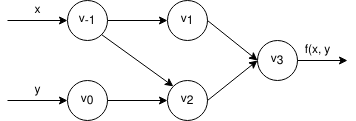
\includegraphics[scale=0.6]{./assets/function_trace.png}
  \caption{Computational graph of $f(x, y) = x^2 + (x - y)$}
  \label{fig:func_trace}
\end{figure}

\begin{table}
  \begin{center}
    \begin{tabular}{ l l l l l | l l l l l }
      \hline
      \multicolumn{5}{l}{Primal trace} & \multicolumn{5}{l}{Tangent trace} \\
      \hline
$v_{-1} $&$=$&$x$&$=$&$2$             &$v'_{-1}$&$=$&$x'$&$=$&$1$ \\
$v_0    $&$=$&$y$&$=$&$1$             &$v'_{0}$&$=$&$y'$&$=$&$0$ \\
      \hline
$v_1    $&$=$&$v_{-1}^2$&$=$&$4$      &$v'_{1}$&$=$&$2*v_{-1}$&$=$&$4$ \\
$v_2    $&$=$&$v_{-1} - v_{0}$&$=$&$1$&$v'_{2}$&$=$&$v'_{-1}-v'_{0}$&$=$&$1$ \\
$v_3    $&$=$&$v_1 + v_2$&$=$&$5$     &$v'_{3}$&$=$&$v'_1 + v'_2$&$=$&$5$ \\
      \hline
$f      $&$=$&$v_3$&$=$&$5$           &$f'$&$=$&$v'_3$&$=$&$5$ \\
      \hline
    \end{tabular}
  \end{center}
  \caption{Primal and tangent traces of $f(x, y) = x^2 + (x - y)$}
  \label{table:func_trace}
\end{table}

\subsection{Denotational semantics}
% A formal semantics of programming language: An introduction

The notion of denotational semantics tries to find underlying mathematical models able to underpin the concepts known in programming languages. The most well-known example is the solution given by Dana Scott and Christopher Strachey\cite{Scott1977} for lambda calculi, also called domain theory.
To be able to formalize non-termination and partiality, they thought to use concepts such as partial orderings and least fixed points\cite{aaby2020}.
In this model, programs are interpreted as partial functions, and recursive computations as taking the fixpoint of such functions.
Non-termination, on the other hand, is formalized as a value \<bottom> that is lower in the ordering relation than any other element.

In our specific case, we try to find a satisfactory model we can use to show that our implementation of forward mode automatic differentiation is correct when applied to a simply-typed lambda calculus.
In the original pen and paper proof of automatic differentiation this thesis is based on, the mathematical models used were diffeological spaces, which are a generalization of smooth manifolds.
For the purpose of this thesis, however, we were able to avoid using diffeological spaces as recursion, iteration and concepts dealing with non-termination and partiality are left out of the scope of this thesis.
\<Coq> has very limited support for domain theoretical models.
There are possible libraries which have resulted from experiments trying to encode domain theoretical models\cite{Benton2009}\cite{Dockins2014}, but these are incompatible with recent versions of \<Coq>.
As a part of its type system, \<Coq> contains a set-theoretical model available under the sort \<Set>, which is satisfactory as the denotational semantics for our language.

Because we use the real numbers as the ground type in our language, we also needed an encoding of the real numbers in Coq. The library for real numbers in \<Coq> has improved in recent times from one based on a completely axiomatic definition to one involving Cauchy sequences\fancyfootnote{https://coq.inria.fr/library/Coq.Reals.ConstructiveCauchyReals.html}. For the purposes of this thesis, however, we needed differentiability as the denotational result of applying the macro operation. Instead of encoding this by hand, we opted for the more comprehensive library \<Coquelicot>\cite{Boldo2015CoquelicotAU}, which contains many general definitions for differentiating functions.


\subsection{Coq}

\<Coq> is a proof assistant based on the calculus of constructions type theory created by Thierry Coquand and G\'{e}rard Huet\cite{Coquand1988}.
In the past 30 years since it has been released, research has contributed to extending the proof assistant with additional features such as inductive and co-inductive data types\cite{Coquand1990}, dependent pattern matching\cite{Sozeau2010} and advanced modular constructions for organizing large mathematical proofs\cite{Sozeau2008}\cite{Mahboubi2013}.

The core of this type theory is based on constructive logic and so many of the laws known in classical logic are not provable.
An example includes the law of the excluded middle, $\forall A, A \vee \neg A$.
In some cases they can, however, be safely added to \<Coq> without making its logic inconsistent. These are readily available in the standard library.
Due to its usefulness in proving propositions over functions, we will make use of the functional extensionality axiom in \<Coq>.

\subsubsection{Language representation}
\label{sec:language_repr}

\begin{figure}
  \begin{mathpar}
    \inferrule*[Right=\textsc{TVar}]
      {elem\ n\ \Gamma = \tau}
      {\Gamma \vdash var\ n : \tau} \and
    \inferrule*[Right=\textsc{TAbs}]
      {(\sigma, \Gamma) \vdash t : \tau}
      {\Gamma \vdash t : \sigma \rightarrow \tau} \\ \and
    \inferrule*[Right=\textsc{TApp}]
      {\Gamma \vdash t1 : \sigma \rightarrow \tau \\
        \Gamma \vdash t2 : \sigma}
      {\Gamma \vdash t1\ t2 : \tau}
  \end{mathpar}
  \label{fig:stlc_infer}
  \caption{Type-inferrence rules for a simply-typed lambda calculus using De-Bruijn indices}
\end{figure}

When defining a simply-typed lambda calculus, there are two main possibilities\cite{plfa2019}.
The arguably simpler variant, known as an extrinsic representation, is traditionally the one introduced to new students learning \<Coq>.
In the extrinsic representation, the terms themselves are untyped and typing judgments are defined separately as relations between the types and terms. A basic example of working with this is given in Software Foundations\cite{Pierce:SF2}.
This, however, required many additional lemmas and machinery to be proved to be able to work with both substitutions and contexts as these are defined separate from the terms.
As an example, the preservation property which states that reduction does not change the type of a term, needs to be proven explicitly.
The other approach, also called an intrinsic representation, makes use of just a single well-typed definition.
Ill-typed terms are made impossible by the type checker.
This representation, while beneficial in the proof load, however complicates much of the normal machinery involved in programming language theory.
One example is how one would define operations such as substitutions or weakening.

But even when choosing an intrinsic representation, the problem of variable binding persists.
Much meta-theoretical research has been done on possible approaches to this problem each with their own advantages and disadvantages.
The POPLmark challenge gives a comprehensive overview of each of the possibilities in various proof assistants\cite{Aydemir2005}.
An example of an approach is the nominal representation where every variable is named.
While this does follow the standard format used in regular mathematics, problems such as alpha-conversion and capture-avoidance appears.

\begin{listing}[h]
  \begin{minted}{coq}
  Inductive ty : Type :=
    | ~unit~ : ~ty~
    | ~\Rightarrow~ : ~ty \rightarrow ty \rightarrow ty~.

  Inductive tm : Type :=
    | var : ~string \rightarrow tm ~
    | abs : ~string \rightarrow ty \rightarrow tm \rightarrow tm~
    | app : ~tm \rightarrow tm \rightarrow tm~.
  \end{minted}
  \caption{Simply typed \lambda-calculus using an extrinsic nominal representation.}
  \label{lst:nominal_stlc}
\end{listing}

The approach used in the rest of this thesis is an extension of the De-Bruijn representation which numbers variables relative to the binding lambda term.
In this representation the variables are referred to as well-typed De-Bruijn indices.
A significant benefit of this representation is that the problems of capture avoidance and alpha equivalence are avoided.
As an alternative, instead of using numbers to represent the distance, indices within the typing context can be used to ensure that a variable is always well-typed and well-scoped.
While the idea of using type indexed terms has been both described and used by many authors\cite{Altenkirch99}\cite{McBride04}\cite{Adams06}, the specific formulation used in this thesis using separate substitutions and rename operations was fleshed out in Coq by Nick Benton, et. al.\cite{Benton2011}, and was also used as one of the examples in the second POPLmark challenge which deals with logical relations\cite{poplmark_reloaded}.
While this does avoid the problems present in the nominal representation, it unfortunately does have some problems of its own.
Variable substitutions have to be defined using two separate renaming and substitution operations.
Renaming is formulated as extending the typing context of variables, while substitution actually swaps the variables for terms.
Due to using indices from the context as variables, some lifting boilerplate is also needed to manipulate contexts.

\begin{listing}[h]
  \begin{minted}{coq}
  Inductive ~\tau \in \Gamma~ : Type :=
    | Top : ~\forall \Gamma \tau, \tau \in (\tau::\Gamma)~
    | Pop : ~\forall \Gamma \tau \sigma, \tau \in \Gamma \rightarrow \tau \in (\sigma::\Gamma)~.

  Inductive tm ~\Gamma \tau~ : Type :=
    | var : ~\forall \Gamma \tau, \tau \in \Gamma \rightarrow tm \Gamma \tau~
    | abs : ~\forall \Gamma \tau \sigma, tm (\sigma::\Gamma) \tau \rightarrow tm \Gamma (\sigma \Rightarrow \tau)~
    | app : ~\forall \Gamma \tau \sigma, tm \Gamma (\sigma \Rightarrow \tau) \rightarrow tm \Gamma \sigma \rightarrow tm \Gamma \tau~.
  \end{minted}
  \caption{Basis of a simply-typed \lambda-calculus using a strongly typed intrinsic formulation.}
  \label{lst:strong_stlc}
\end{listing}

% TODO: Work out how substitutions work

\subsubsection{Dependently-typed programming in Coq}

In \<Coq>, one can normally write function definitions using either case-analysis as is done in other functional languages, or using \<Coq>'s tactics language.
Using the standard case-analysis functionality can cause the code to be complicated and verbose, even more so when proof terms are present in the function signature.
This has been caused by the previously poor support in Coq for dependent pattern matching.
Using the return keyword, one is able to vary the result type of a match expression. But due to requirement Coq used to have that case expressions be syntactically total, this could be very annoying to work with.
One other possibility would be to write the function as a relation between its input and output.
This also has its limitations as you then lose computability as Coq treats these definitions opaquely. In this case the standard \<simpl> tactic which invokes \<Coq>'s reduction mechanism is not able to reduce instances of the term.
This often requires the user to write many more proofs to be able to work with the definitions.

As an example, we will work through defining a length indexed list and a corresponding head function limited to lists of length at least one in Snippet~\ref{lst:dt_ilist}.
Using the \<Coq> keyword return, it is possible to let the return type of a match expressions depend on the result of one of the type arguments.
This makes it possible to define an auxiliary function which, while total on the length of the list, has an incorrect return type. It namely returns the type unit if the input list had the length zero.
We can then use this auxiliary function in the actual head function by specifying that the list has length at least one.
It should be noted that more recent versions of Coq do not require that case expressions be syntactically total, so specifying that the input list has a length of at least zero is enough to eliminate the requirement for the zero-case.

\begin{listing}
  \begin{minted}{coq}
  Inductive ilist : ~Type \rightarrow nat \rightarrow Type~ :=
    | nil : ~\forall A, ilist A 0~
    | cons : ~\forall A n, A \rightarrow ilist A n \rightarrow ilist A (S n)~

  Definition hd' {A} n (ls : ilist A n) :=
    match ls in (ilist A n) return
      (match n with
      | O => unit
      | S _ => A end) with
    | nil => tt
    | cons h _ => h
  end.

  Definition hd {A} n (ls : ilist A (S n)) : A := hd' n ls.
  \end{minted}
  \caption{Definition of a length indexed list and hd using the return keyword, adapted from Certified Programming with Dependent Types\cite{ChlipalaCPDT}.}
  \label{lst:dt_ilist}
\end{listing}

Mathieu Sozeau introduces an extension to \<Coq> via a new keyword \<Program> which allows the use of case-analysis in more complex definitions\cite{Sozeau2006}\cite{Sozeau2007}.
To be more specific, it allows definitions to be specified separately from their accompanying proofs, possibly filling them in automatically if possible.
While this does improve on the previous situation, using the definitions in proofs can often be unwieldy due to the amount of boilerplate introduced.
This makes debugging error messages even harder than it already is in a proof assistant. This approach was used by Benton in his formulation of strongly typed terms.

Sozeau further improves on this introducing a method for user-friendlier dependently-typed pattern matching in \<Coq> in the form of the \<Equations> library\cite{Sozeau2010}\cite{Sozeau2019}.
This introduces \<Agda>-like dependent pattern matching with with-clauses.
It does this by using a notion called coverings, where a covering is a set of equations such that the pattern matchings of the type signature are exhaustive.
There are two main ways to integrate this in a dependently typed environment, externally where it is integrated as high-level constructs in the pattern matching core as \<Agda> does it, or internally by using the existing type theory and finding witnesses of the covering to prove the definition correct, which is the approach used by Sozeau.
Due to the intrinsic typeful representation this paper uses, much of this was invaluable when defining the substitution operators as the regular type checker in Coq often had difficulty unifying dependently typed terms in certain cases.

\begin{listing}
  \begin{minted}{coq}
  Equations hd {A n} (ls : ilist A n) (pf : n <> 0) : A :=
  hd nil pf with pf eq_refl := {};
  hd (cons h n) _ := h.
  \end{minted}
  \caption{Definition of hd using \<Equations>}
  \label{lst:dt_ilist_hd_equations}
\end{listing}


\subsection{Logical relations}

Logical relations is a technique often employed when proving programming language properties of statically typed languages\cite{skorstengaard2019introduction}. There are two main ways they are used, namely as unary and binary relations.
Unary logical relations, also known as logical predicates, are predicates over single terms and are typically used to prove language characteristics such as type safety or strong normalization.
Binary logical relations on the other hand are used to prove program equivalences, usually in the context of denotational semantics as we will do.
There have been many variations on the versatile technique from syntactic step-indexed relations which have been used to solve recursive types\cite{Ahmed2006}, to open relations which enable working with terms of non-ground type\cite{barthe2020versatility}\cite{huot2020correctness}.
Logical relations in essence are relations between terms defined by induction on their types.
A logical relations proof consists of 2 main steps.
The first states the terms for which the property is expected to hold are in the relation, while the second states that the property of interest follows from the relation.
The second step is easier to prove as it usually follows from the definition of the relation. The first on the other hand, will often require proving a generalized variant, called the fundamental property of the logical relation.
In most cases this requires that the relation is correct with respect to applying substitutions.

A well-known logical relations proof is the proof of strong normalization of well-typed terms, which states that all terms eventually terminate.
An example of a logical relation used in such a proof using the intrinsic strongly-typed formulation is given in Snippet~\ref{lst:sn_logical_relation}.
Noteworthy is the case for function types, which indicates that an application should maintain the strongly normalization property.
If one were to attempt the proof of strong normalization without using logical relations, they would get stuck in the cases dealing with function types.
More specifically when reducing an application, the induction hypothesis is not strong enough to prove that substituting the argument into the body of the abstraction also results in a terminating term.
The proof given in the paper this thesis is based on, is a logical relations proof on the denotation semantics using diffeological spaces as its domains\cite{huot2020correctness}.
A similar, independent proof of correctness was given by Barthe, et. al.\cite{barthe2020versatility} using a syntactic relation on the operational semantics.

\begin{listing}
  \begin{minted}{coq}
    Equations SN {~\Gamma~} ~\tau~ (t : ~tm \Gamma \tau~): Prop :=
    SN unit t := halts t;
    SN ~(\tau \Rightarrow \sigma)~ t := halts t ~$\wedge$~
      ~(\forall (s : tm \Gamma \tau), SN \tau s \rightarrow SN \sigma (app \Gamma \sigma \tau t s))~;
  \end{minted}
  \caption{Example of a logical predicate used in a strong normalizations proof in the intrinsic strongly-typed formulation}
  \label{lst:sn_logical_relation}
\end{listing}

\section{Formalizing Forward-Mode AD}
  We will work out the formalization of automatic differentiation using a source code translating macro in the following sections.
  We start from a base simply-typed lambda calculus extended with product types and incrementally add both sum and array types.

  \subsection{Simply Typed Lambda Calculus}
  % Talk about simply typed lambda calculus,
  % Something about Λ_δ^{+, *, R}
  % Give examples of functions
  % talk about denotations and
  As mentioned in background section \ref{sec:language_repr}, we will make use of De-Bruijn indices in a intrinsic representation to formulate our language.
  Our base language consists of the typed lambda calculus with products and real numbers as ground type, $\Lambda_{\delta}^{\times, \rightarrow, R}$.
  As operations on the real numbers we include both addition and multiplication which are also the functions in $\delta$.

  Both the language constructs and the typing rules for this language are standard for a simply typed lambda calculus, as shown in \ref{fig:base_infer}.
  As expected we include variables, applications and abstractions in the \<var>, \<app> and \<abs> constructors.
  Product types are added to the language in the form of binary projections, \<first> and \<second> to fetch respectively the first and second components of \<tuple>s.
  For real numbers, \<rval> is used to introduce constants and \<add> and \<mul> will be used to respectively encode addition and multiplication.

  \begin{figure}
    \begin{mathpar}
      \inferrule*[Right=\textsc{TVar}]
        {elem\ n\ \Gamma = \tau}
        {\Gamma \vdash var\ n : \tau} \and
      \inferrule*[Right=\textsc{TAbs}]
        {(\sigma, \Gamma) \vdash t : \tau}
        {\Gamma \vdash abs\ t : \sigma \rightarrow \tau} \\ \and
      \inferrule*[Right=\textsc{TApp}]
        {\Gamma \vdash t1 : \sigma \rightarrow \tau \\
          \Gamma \vdash t2 : \sigma}
        {\Gamma \vdash app\ t1\ t2 : \tau} \\ \and
      \inferrule*[Right=\textsc{TTuple}]
        {\Gamma \vdash t1 : \tau \\
          \Gamma \vdash t2 : \sigma}
        {\Gamma \vdash tuple\ t1\ t2 : \tau \times \sigma} \\ \and
      \inferrule*[Right=\textsc{TFst}]
        {\Gamma \vdash t : \tau \times \sigma}
        {\Gamma \vdash first\ t : \tau} \and
      \inferrule*[Right=\textsc{TSnd}]
        {\Gamma \vdash t : \tau \times \sigma}
        {\Gamma \vdash second\ t : \sigma} \\ \and
      \inferrule*[Right=\textsc{TRval}]
        {r \in \<R>}
        {\Gamma \vdash rval\ r : R} \\ \and
      \inferrule*[Right=\textsc{TAdd}]
        {\Gamma \vdash r1 : R \\
          \Gamma \vdash r2 : R \\ }
        {\Gamma \vdash add\ r1\ r2 : R} \and
      \inferrule*[Right=\textsc{TMull}]
        {\Gamma \vdash r1 : R \\
        \Gamma \vdash r2 : R \\ }
      {\Gamma \vdash mul\ r1\ r2 : R} \and
    \end{mathpar}
    \caption{Type-inferrence rules for $\lambdaBase$}
    \label{fig:base_infer}
  \end{figure}

  % How we translated this into the well-typed intrinsic representation
  These can be translated into Coq definitions in a straigtforward manner, with each case keeping track of both how the typing context and types change.
  In the \<var> case we need some way to determine what type the variable is referencing.
  Like many others previously\cite{Benton2011}\cite{Coquand1994}, instead of using numbers accompanied with a proof, we make use of an inductively defined type evidence to type our variables as shown in \ref{lst:strong_stlc}.
  The cases for \<app> and \<abs> are as expected, where variables in the body of abstraction are able to reference their respective arguments.

  In the original proof by Huot, Staton, and \Vakar{} \cite{huot2020correctness}, they make use of n-ary products accompanied with pattern matching expressions. We opted to implement binary projection products, as they are conceptually simpler while still retaining much of the same functionality expected with product types.

  \begin{listing}
    \begin{minted}{coq}
  Definition Ctx : Type := list ty.

  Inductive tm ~(\Gamma : Ctx) : ty \rightarrow Type~ :=
    (* Base STLC *)
    | var : ~forall \tau,
      \tau ∈ \Gamma \rightarrow tm \Gamma \tau~
    | app : ~forall \tau \sigma,
      tm \Gamma (\sigma \Rightarrow \tau) \rightarrow
      tm \Gamma \sigma \rightarrow
      tm \Gamma \tau~
    | abs : ~forall \tau \sigma,
      tm (\sigma::\Gamma) \tau \rightarrow tm \Gamma (\sigma \Rightarrow \tau)~

    (* Operations on real numbers *)
    | const : ~R \rightarrow tm \Gamma Real~
    | add : ~tm \Gamma Real \rightarrow tm \Gamma Real \rightarrow tm \Gamma Real~
    | mul : ~tm \Gamma Real \rightarrow tm \Gamma Real \rightarrow tm \Gamma Real~

    (* Binary projection products *)
    | tuple : ~forall {\tau \sigma},
      tm \Gamma \tau \rightarrow
      tm \Gamma \sigma \rightarrow
      tm \Gamma (\tau \times \sigma)~
    | first : ~forall {\tau \sigma}, tm \Gamma (\tau \times \sigma) \rightarrow tm \Gamma \tau~
    | second : ~forall {\tau \sigma}, tm \Gamma (\tau \times \sigma) \rightarrow tm \Gamma \sigma~
    \end{minted}
    \caption{\<Coq> definition of the base lambda calculus}
    \label{lst:stlc_base}
  \end{listing}

  We use the same inductively defined macro on types and terms to implement forward-mode automatic differentiation as used by many previous authors\cite{huot2020correctness}\cite{barthe2020versatility}\cite{Shaikha2019}.
  The forward-mode macro $\D$ keeps track of both primal and tangent traces using tuples as respectively the first and second subcomponents.
  In most cases, the macro simply preserves the structure of the language.
  In the cases for real numbers such as addition and multiplication, the appropriate implementation corresponding to the derivative needs to be given.

  \begin{align*}
    \D(\<R>) &= \<R> \times \<R>
      & \D(n) &= (n, 0) \\
    \D(\tau \times \sigma) &= \D(\tau) \times \D(\sigma)
      & \D(n + m) &= (n + m, n' + m') \\
    \D(\tau \rightarrow \sigma) &= \D(\tau) \rightarrow \D(\sigma)
      & \D(n * m) &= (n * m, n' * m + m' * n)
    \label{eqn:macro_base}
  \end{align*}

  This is implemented by destructing recursive calls to $\<D>$ to access the syntactic counterparts of the primal and tangent denotations.
  The \<Coq> implementation requires seperate definitions for types, typing contexts and terms, as shown in \ref{lst:macro_base}.
  Note that applying the macro to a variable does nothing as we already apply the macro to the typing context, so variable implicitly reference macro-applied values.

  \begin{listing}
    \begin{minted}{coq}
    \end{minted}
    \caption{Forward-mode macro on the base simply-typed lambda calculus.}
    \label{lst:macro_base}
  \end{listing}

  Due to restricting our language to be total and excluding constructs related to partiality such as general recursion and iteration, it suffices to give our language a set-theoretic denotational semantics. Well-typed terms $\Gamma \vdash t : \tau$ will denotate to functions $\llbracket \Gamma \rrbracket \rightarrow \llbracket \tau \rrbracket$.

  \begin{equation}
    \llbracket t \rrbracket =
      \left\{
        \begin{array}{ll}
          \lambda x. lookup\ \llbracket v \rrbracket\ x
            & : t = \<var>\ v \\
          \lambda x. (\llbracket t1 \rrbracket(x)) (\llbracket t2 \rrbracket(x))
            & : t = \<app>\ t1\ t2 \\
          \lambda x y. \llbracket t \rrbracket(y :: x)
            & : t = \<abs>\ t \\
          const\ n
            & : t = \<rval>\ n \\
          \lambda x. \llbracket t1 \rrbracket(x) + \llbracket t2 \rrbracket(x)
            & : t = \<add>\ t1\ t2 \\
          \lambda x. \llbracket t1 \rrbracket(x) * \llbracket t2 \rrbracket(x)
            & : t = \<mul>\ t1\ t2 \\
          \lambda x. (\llbracket t1 \rrbracket(x), \llbracket t2 \rrbracket(x))
            & : t = \<tuple>\ t1\ t2 \\
          \lambda x. let\ (x, y) = \llbracket t \rrbracket(x)\ in\ x
            & : t = \<first>\ t \\
          \lambda x. let\ (x, y) = \llbracket t \rrbracket(x)\ in\ y
            & : t = \<second>\ t \\
        \end{array}
      \right.
  \label{eqn:lr_base}
  \end{equation}

  For any type $\tau$, simply swap out the syntactic type to its corresponding \<Coq> variant in \<Type>.
  We denotate our typing contexts $\Gamma$, lists of types, as heterogeneous lists containing their corresponding denotations.
  The specific implementation of heterogeneous lists used, correspond to the one given by Adam Chlipala\cite{ChlipalaCPDT}.
  When working through giving the constructs in our language the proper denotations, most of the cases are straigtforward.
  Notable is the case for variables, where we made use of an inductively defined evidence to type our terms.
  As denotations, these evidences wil correspond to lookups into our heterogeneous lists to their appropriate types.

  \begin{listing}
    \begin{minted}{coq}
    \end{minted}
    \caption{Denotatonal semantics for the base simply-typed lambda calculus.}
    \label{lst:denotation_base}
  \end{listing}

  % In the section denotation
  % Explain expressiveness of base language
  % Work out examples
  As mentioned by by Barthe, et. al.\cite{barthe2020versatility}, this small calculus, $\lambdaBase$, accompanied with a very simple denotational semantics is expressive enough to encode all higher-order polynomial functions containing the addition and multiplication operators.

  \begin{example}[Square]
    $abs\ (mul\ (var\ Top)\ (var\ Top))$ denotates to the square function $\lambda x. x * x$.
    \begin{proof}
      This follows from the definition of our denotation functions.
      \begin{align*}
        \llbracket abs\ &(mul\ (var\ Top)\ (var\ Top)) \rrbracket\ [] \\
          &\equiv \lambda x.
            \llbracket mul\ (var\ Top)\ (var\ Top) \rrbracket\ [x] \\
          &\equiv \lambda x.
            \llbracket var\ Top \rrbracket\ [x] *
              \llbracket var\ Top \rrbracket\ [x] \\
          &\equiv \lambda x. x * x \qedhere
      \end{align*}
    \end{proof}
  \end{example}

  % TODO: give reasonable examples

  As we work with denotations, smooth functions $f : \<R>^n -> \<R>$ can be interpreted as the denotations of a corresponding syntactic term $x_1, \dots, x_n \vdash t : R$.
  The idea here is that the free variables in the term $t$ denote the usages of the parameters of the function and as such are restricted to terms of type $R$.
  Note that while both the arguents and result type of $t$ are restricted to $R$, $t$ itself can contain higher order types.

  Although Barthe, et. al.\cite{barthe2020versatility} gave a syntactic proof of correctness of the macro, our proof follows the more denotational style of proof given by Huot, Staton and \Vakar{}\cite{huot2020correctness}.
  We state correctness as the denotation of a macro-applied term will give a pair of both the original function the term represents along with its corresponding derivative.

  The proof of correctness will follow a logical relations argument.Intuitively, the relation will encapsulate idea that derivability is preserved over higher-order types.
  We define a type-indexed logical relation between denotations of both terms and their macro-applied variants, so for any type $\tau$, $S_\tau$ is the relation between functions $R \rightarrow \llbracket \tau \rrbracket$ and $R \rightarrow \llbracket \D(\tau) \rrbracket$.

  \begin{equation}
    S_\tau(f, g) =
      \left\{
        \begin{array}{ll}
          smooth\ f \wedge
            g = \lambda x. (f(x), \frac{\partial f}{\partial x}(x))
            & : \tau = R \\
          \exists f_1, f_2, g_1, g_2,
            & : \tau = \sigma \times \rho \\
            \;\;\;\;S_\sigma(f_1, f_2), S_\sigma(g_1, g_2). \\
            \;\;\;\;f = \lambda x. (f_1(x), g_1(x)) \wedge \\
            \;\;\;\;g = \lambda x. (f_2(x), g_2(x)) \\
          \forall f_1, f_2.
            & : \tau = \sigma \rightarrow \rho \\
            \;\;\;\;S_\sigma(f_1, f_2) \Rightarrow \\
            \;\;\;\;S_\rho(\lambda x. f(x)(f_1(x)),\lambda x. f(x)(f_2(x)))
        \end{array}
      \right.
  \label{eqn:lr_base}
  \end{equation}

  The next step involves proving that syntactically well-typed terms are semantically correct.
  In other words, the relation is valid for any term $x_1, \dots, x_n \vdash t : \tau$ and argument function $f : R \rightarrow R^n$ such that $S_\tau(\llbracket t \rrbracket \circ f, \llbracket \D(t) \rrbracket \circ \D_f \circ f)$.
  Note the need to apply a function $\D_f$ which essentially accompanies each argument supplied by $f$ with its accompanying derivative, $0$.

  Proving this statement directly by induction on the typing derivation, however, does not work.
  As expected in a logical relations proof, the indicative issue lies in both the case for applications and abstractions.
  To make this work, the correctness statement needs to be generalized to arbitrary contexts and implicitly, substitutions.

  If this were a syntactic proof, one would need to show that relation is preserved when applying substitutions consisting of arbitrary terms, possibly containing higher-order constructs.
  In this style of proof, the same concept needs to be incorporated in the argument function $f$, which intuitively speaking, supplies the terms referenced by variables through the typing context.

  % TODO: attempt to do this?

  To prove this statement, it first needs to be generalized to arbitrary substitutions.
  The key in formulating these denotationally lies in what was previously the argument function $f : R \rightarrow R^n$.
  Previously the function was used to indicate the open variables or function arguments.
  If generalized to $\Gamma = x_1 : \tau_1, \dots, x_n : \tau_n$, this same function could be seen as a function which supplies terms foreach open variable $x_1, \dots, x_n$ with their appropriate types.
  So the argument function now becomes the pair of functions $s : R \rightarrow \llbracket \Gamma \rrbracket$ and $s' : R \rightarrow \llbracket \D(\Gamma) \rrbracket$.
  Note that the functions $s$ and $s'$ are built out of the denotations of terms such that these same denotations follow the logical relation (\ref{eqn:lr_base}) for our language.
  We phrase this requirement as a definition.

  \begin{definition}(Instantiation)
    Substitutional functions $s : R \rightarrow \llbracket \Gamma \rrbracket$ and $s' : R \rightarrow \llbracket \D(\Gamma) \rrbracket$ are inductively instantiated such that they follow
    \begin{equation}
      inst_\Gamma(f, g) =
        \left\{
          \begin{array}{ll}
            f = const([]) \wedge g = const([])
              & : \Gamma = [] \\
            \forall s, s'.
              & : \Gamma = (\tau :: \Gamma') \\
              \;\;\;\;inst_{\Gamma'}(s, s') \wedge S_\tau(f, g)
          \end{array}
        \right.
    \label{eqn:lr_base}
    \end{equation}
  \end{definition}

  Using this notion of substitution instantiations we can now formulate our substitution lemma.

  \begin{lemma}[Substitution]
    If for any well-typed term $\Gamma \vdash t : \tau$, and instantiation functions $s : R \rightarrow \llbracket \Gamma \rrbracket$ and $s' : R \rightarrow \llbracket \D(\Gamma) \rrbracket$ such that they follow $inst_\Gamma(s, s')$ then $S_\tau(\llbracket t\rrbracket \circ s, \llbracket \D(t)\rrbracket \circ s')$.
  \end{lemma}

  \begin{proof}
    This is proven by induction on the typing derivation of $t$.
    Unless otherwise specified, the type of $s$ and $s'$ are respectively $R \rightarrow \llbracket \Gamma \rrbracket$ and $R \rightarrow \llbracket \D(\Gamma) \rrbracket$.
    \begin{enumerate}
      \item (\<var>)
        Prove: $S_\tau(\llbracket var\ v \rrbracket \circ s, \llbracket \D(var\ v) \rrbracket \circ s)$.

        Proceed by induction on the type evidence $v$.
        \begin{itemize}
          \item(\<Top>) Base case

          Prove: $S_\tau(\llbracket var\ Top \rrbracket \circ s, \llbracket \D(var\ Top) \rrbracket \circ s')$

          In this case the referenced $\tau$ exists at the top of the list.
          So both $\llbracket var\ Top \rrbracket$ and $\llbracket \D(var\ Top) \rrbracket$ denotate to fetching the top term.
          This is now proven by definition of $inst$, which states that the the term is semantically well-typed.

          \item(\<Pop>) Induction step

          Prove: $S_\tau(\llbracket var\ (Pop\ v) \rrbracket \circ s, \llbracket \D(var\ (Pop\ v)) \rrbracket \circ s')$, where $s : R \rightarrow \llbracket \sigma :: \Gamma \rrbracket$ and $s' : R \rightarrow \llbracket \D(\sigma :: \Gamma) \rrbracket$.

          The induction hypothesis states $\forall (f : R \rightarrow \llbracket \Gamma \rrbracket), (g : R \rightarrow \llbracket \D(\Gamma) \rrbracket). S_\tau(\llbracket var\ v \rrbracket \circ f, \llbracket \D(var\ v) \rrbracket \circ g)$

          Note that the \<var> term now denotates to ignoring the arbitrary unrelated type $\sigma$ and looking up $v$ in the rest of the list $\Gamma$.
          So $S_\tau(\llbracket var\ v \rrbracket \circ tl \circ s, \llbracket \D(var\ v) \rrbracket \circ tl \circ s')$, which is proven using the induction hypothesis by respectively instantiating $f$ and $g$ as $tl \circ s$ and $tl \circ s'$. \qed
        \end{itemize}
      \item (\<app>)

        Prove: $S_\tau(\llbracket app\ t_1\ t_2 \rrbracket \circ s, \llbracket \D(app\ t_1\ t_2) \rrbracket \circ s')$

        Induction hypotheses:
        \begin{enumerate}
          \item \label{eqn:subst_ih_app1}$S_{\sigma\rightarrow\tau}(\llbracket t_1 \rrbracket \circ s, \llbracket \D(t_1) \rrbracket \circ s')$
          \item \label{eqn:subst_ih_app2}$S_{\sigma}(\llbracket t_2 \rrbracket \circ s, \llbracket \D(t_2) \rrbracket \circ s')$
        \end{enumerate}

        First it is useful to rewrite the induction hypothesis \ref{eqn:subst_ih_app1} in a more usable format. Rewrite the statement using the definition of $S$ at function types.

        \begin{align*}
          S&_{\sigma\rightarrow\tau}(\llbracket t_1 \rrbracket \circ s, \llbracket \D(t_1) \rrbracket \circ s') \\
            & \Vdash \text{(Definition of \circ)} \\
            & S_{\sigma\rightarrow\tau}(\lambda x. \llbracket t_1 \rrbracket(s(x)), \lambda x. \llbracket \D(t_1) \rrbracket(s'(x))) \\
            & \Vdash \text{(Definition of $S_{\rightarrow}$)} \\
            & \forall f_1, f_2.
              S_{\sigma}(f1, f2) \rightarrow \\
            &S_\tau(\lambda x. (\llbracket t_1 \rrbracket(s(x)))(f_1(x)), \lambda x. (\llbracket \D(t_1) \rrbracket(s'(x)))(f_2(x)))
        \end{align*}

        The case for \<app> is now proven by applying the induction hypothesis \ref{eqn:subst_ih_app1} for the function term using the induction hypothesis \ref{eqn:subst_ih_app2} for the argument term to satify its premise.

        \begin{align*}
          S&_\tau(\llbracket app\ t_1\ t_2 \rrbracket \circ s, \llbracket \D(app\ t_1\ t_2) \rrbracket \circ s') \\
            &\Vdash \text{(Definition of $\D$)}\\
            & S_\tau(\llbracket app\ t_1\ t_2 \rrbracket \circ s, \llbracket app\ \D(t_1)\ \D(t_2) \rrbracket \circ s') \\
            &\Vdash \text{(Definition of \circ)}\\
            & S_\tau(\lambda x. \llbracket app\ t_1\ t_2 \rrbracket (s (x)), \lambda x. \llbracket app\ \D(t_1)\ \D(t_2) \rrbracket (s' (x))) \\
            &\Vdash \text{(Definition of $\llbracket \rrbracket$)}\\
            & S_\tau(\lambda x. (\llbracket t_1\ \rrbracket(s(x))) (\llbracket t_2 \rrbracket(s(x))),\lambda x. (\llbracket \D(t_1)\ \rrbracket(s'(x))) (\llbracket \D(t_2) \rrbracket(s'(x))) \\
            &\Vdash \text{(Induction hypothesis \ref{eqn:subst_ih_app1})}\\
            & S_{\sigma}(\lambda x. \llbracket t_2 \rrbracket (s(x)), \lambda x. \llbracket \D(t_2) \rrbracket \circ (s'(x))) \\
            &\Vdash \text{(Induction hypothesis \ref{eqn:subst_ih_app2})} \\
        \end{align*} \qed
      \item (\<abs>)

        Prove: $S_{\sigma\rightarrow\tau}(\llbracket abs\ t \rrbracket \circ s, \llbracket \D(abs\ t) \rrbracket \circ s')$

        Induction hypothesis:
        \begin{enumerate}
          \item \label{eqn:subst_ih_abs} $S_\sigma(\llbracket t \rrbracket \circ s, \llbracket \D(t) \rrbracket \circ s')$, where $s : R \rightarrow \llbracket \sigma::\Gamma \rrbracket$ and $s' : R \rightarrow \llbracket \sigma::\Gamma \rrbracket$
        \end{enumerate}

        As is the case for \ref{eqn:subst_ih_app1}, simplify the goal statement using the definition of $S_\rightarrow$. So the proof obligation now becomes.

        Prove: $S_{\tau}(\lambda x. (\llbracket abs\ t \rrbracket (s(x)))(f_1(x)), \lambda x. (\llbracket \D(abs\ t) \rrbracket (s'(x)))(f_2(x)))$

        Assume:
        \begin{enumerate}
          \item $f_1 : R \rightarrow \llbracket \sigma \rrbracket$
          \item $f_2 : R \rightarrow \llbracket \D(\sigma) \rrbracket$
          \item \label{eqn:subst_ass_abs3} $S_\sigma(f_1, f_2)$
        \end{enumerate}

        The proof proceeds by rewriting the goal until we can apply the induction hypothesis.
        Note that the assumption \ref{eqn:subst_ass_abs3}: $S_\sigma(f_1, f_2)$ ensures that the requirement of $inst_{\sigma::\Gamma}$ in the induction hypothesis \ref{eqn:subst_ih_abs} is satisfied.

        \begin{align*}
          S&_{\tau}(\lambda x. (\llbracket abs\ t \rrbracket (s(x)))(f_1(x)), \lambda x. (\llbracket \D(abs\ t) \rrbracket (s'(x)))(f_2(x))) \\
            &\Vdash \text{(Definition of $\D$)}\\
            & S_{\tau}(\lambda x. (\llbracket abs\ t \rrbracket (s(x)))(f_1(x)), \lambda x. (\llbracket abs\ \D(t) \rrbracket (s'(x)))(f_2(x))) \\
            &\Vdash \text{(Definition of $\llbracket \rrbracket$)}\\
            & S_{\tau}(\lambda x. (\llbracket t \rrbracket (f_1(x) :: s(x))), \lambda x. (\llbracket \D(t) \rrbracket (f_2(x) :: s'(x)))) \\
            &\Vdash \text{(Induction hypothesis \ref{eqn:subst_ih_app1})}
        \end{align*} \qed

      \item (\<rval>)

      Prove: $S_{R}(\llbracket rval\ n \rrbracket \circ s, \llbracket \D(rval\ n) \rrbracket \circ s')$

      This is proven by nothing that the corresponding denotations of \<rval> are constant functions, which are both smooth and whose derivatives are equal to $0$.

      \begin{align*}
        S&_{\tau}(\llbracket rval\ n \rrbracket \circ s, \llbracket \D(rval\ n) \rrbracket \circ s') \\
        &\Vdash \text{(Definition of $\D$)}\\
        &S_{\tau}(\llbracket rval\ n \rrbracket \circ s, \llbracket tuple\ (rval\ n)\ (rval\ 0) \rrbracket \circ s') \\
        &\Vdash \text{(Definition of $\llbracket\rrbracket$)}\\
        &S_{\tau}(const\ n, (const\ n, const\ 0)) \\
        &\Vdash \text{(Definition of $S_R$)}\\
        &smooth\ (const\ n) \wedge
          const\ 0 = \sfrac{\partial{const\ n}}{\partial{x}} \\
        &\Vdash \text{(split goals: goal 1)}\\
        &\;\;\;smooth\ (const\ n) \\
        &\;\;\;\Vdash \text{($f(x) = n$ is continuously differentiable)}\\
        &\Vdash \text{(split goals: goal 2)}\\
        &\;\;\;const\ 0 = \sfrac{\partial{const\ n}}{\partial{x}} \\
        &\;\;\;\Vdash \text{(if $f(x) = n$, then $\sfrac{\partial{f}}{\partial{x}} = 0$)}
      \end{align*} \qed
      \item (\<add>)
      \item (\<mul>)
      \item (\<tuple>)
      \item (\<first>)
      \item (\<second>)
    \end{enumerate}
  \end{proof}

  \begin{theorem}[Macro correctness]
    For any term $x_1 : R, ..., x_n : R \vdash t : R$, $\D(t)$ gives the dual number representation of $\llbracket t \rrbracket$.
  \end{theorem}

  \begin{proof}

  \end{proof}



  \subsection{Adding Sums and Primitive Recursion}
  \subsection{Arrays}
\section{Optimization}
  \subsection{Program Transformations}
\section{Reverse-Mode AD}
\section{Discussion}
  \subsection{Problems}
  \subsection{Future Work}
\section{Conclusion}

\appendix
\section{Language Definitions}
\section{Forward-Mode Macro}
\section{Denotations}
\printbibliography
\makeatother
\end{document}